\chapter{Materials and Methods}
%Erklären welche Methoden beleuchtet werden
%Pipeline mit mehr details einfügen 
%Vielleicht erklären, warum in silico datensatz?
A network inference problem is a classification problem in which edges in a network are classified as being true or false. In general, after selecting the parameter for inferring a network an experimental data set is divided up into two sets, a training and a test set. On the training set the network is inferred multiple times. The inferred network with the lowest error is tested by the test set. Experimental settings often contain batch effects from the laboratory and much of information (e.g. many nodes, pertubations by adding drugs), such that assessing an inference method by an \textit{in silico} data set is useful. An \textit{in silico} data set is a computational simulated data set containing no batch effects and with less nodes and pertubations representing a simplified version of the training data. Hence, by an \textit{in silico} data set the parameters of inferring a network can be analyzed more easily. In this work an \textit{in silico} data set is created from E.Coli for investigating the runtime and influence of the in degree of a network on the inference algorithms performance. Additionally a second \textit{in silico} data set derived from the cell cycle network which is used to assess the performance of the inference algorithms relating to the cluster depth in binarization of the continous data and the number of sample points. The training data set is an experimental data set from the Dream8 Challenge. This challenge comes along with a test data set used as a gold standard with the same abundance of nodes as in the training set, but less sample points which makes it hard for the inference algorithms to perform. In this context a gold standard is a network being close to the structure of an 'unseen' network $G(X,A)$ the inference algorithms aims to infer. Thus the performance of an algorithms is achieved by testing an inferred network $G'(X',A')$ against a gold standard network $G(X,A)$. Often a gold standard network is a combination of prior knowledge from literature with previously inferred networks. In this work two gold standard networks are selected for the network evaluation in the Dream8 Challenge described in chapter 3.\\ 
%Quelle?Von Dream8 Paper? 
The Figure 2.1 shows a raw structure of a pipeline for inferring and evaluating a network. Both \textit{in silico} and experimental data are binarized, redundant transitions are removed and an inference algorithm is applied. The network with the lowest error is scored against a gold standard network. 
%Quellen einfügen?
%Graphik einfügen
\begin{figure}[H]
\centering

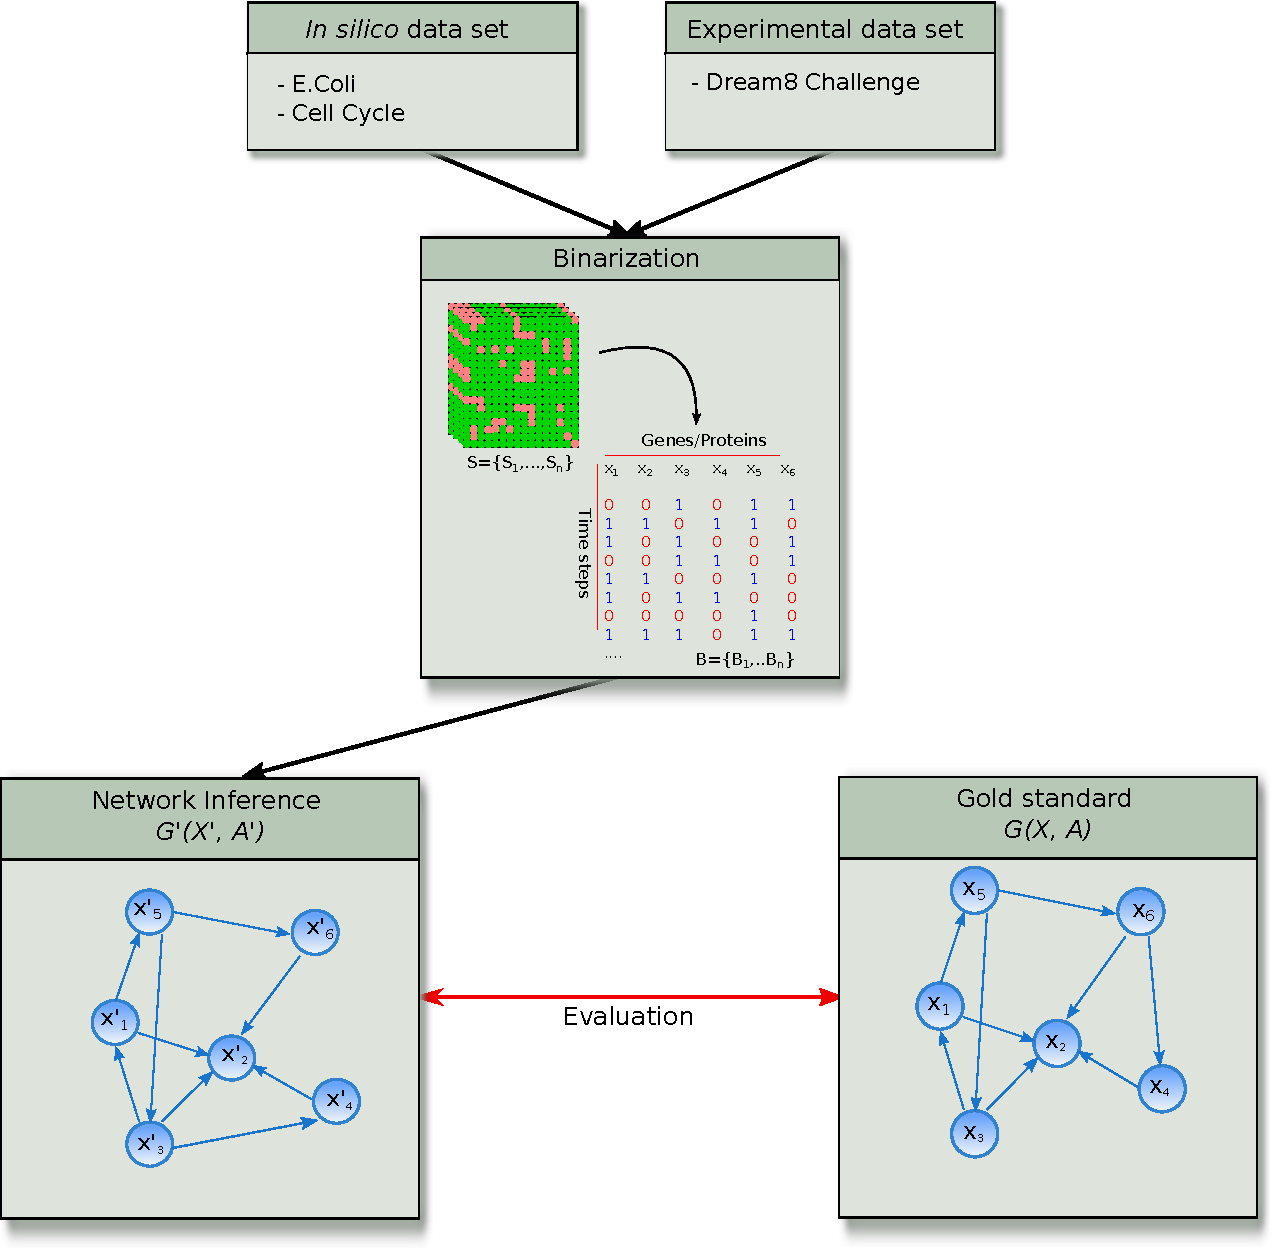
\includegraphics[width=0.6\textwidth]{./Bilder/IntroductionPipeline2.pdf}
\caption[General Pipeline]{\textbf{General Pipeline.} Continous data sets $S$ of \textit{in silico} data sets and an experimental data set are discretisized to binary trajectories $B$. The inferred network $G'$ is scored against a gold standard network $G'$. }
\label{fig:General Pipeline}
\end{figure} 



\section{Inferencealgorithms}
%Warum wählen wir hier den Boolean Approach?
%Baysian networks,Boolean regulatory networks, Ordinary differential equation models and Neural networks, regression
%Determinische und PBN models erklären
Different approaches of inferring networks are known capturing several advantages and limitations.  
It is worhtwhile to find a good trade-off between simplicity, scalability, expressiveness and finding the abstraction level for a significant network. 
%\citep{Kitano1662}
Many inference algorithms are known based on different computational models like the Bayesian approach , the ordinary diffential equation approach (ODE), the artificial neural networks )(ANN) and the Boolean model (BN).%\citep{Lähdesmäki2003}\\
A Bayesian model is a graph-based model of joint multivariate probability distributions that captures properties of conditional independence between variables.\\
%(In other words given a gene A and a gene B and a third gene C, then A and B are conditionally independent given C iif, given knowledge that C occurs, knowledge of wether A occurs provides no information on the likelihood of B occuring,and knowledge of wether B occurs provides no information on the likelihood of A occuring.)
The system of differential equations (ODE's) creates networks in consideration with the kinetic properties of a biological system. An ODE is a powerful and flexible model to describe complex relations among components. But the higher the complexity of an unseen network is the more challenging it is to determine an appropriate set of equations which describe the network.
% \citep{article}\\
Artificial Neural networks gather their knowledge by detecting patterns and relationships in data and learn through experience. An ANN is constructed by weighted processing elements which constitute the neural layers and are organized in layers. Thus the behaviour of a ANN is determined by a transition function of each variable (neuron), by a learning rule and by the architecture itself. A big advantage, no previous knowledge is needed %\citep{AGATONOVICKUSTRIN2000717}.\\
Boolean Models are simple Boolean Networks which are well known and an appropriate strategy of inferring the structure and the dynamics behaviour of complex data. A big advantage is that Boolean Network Models do not need any information about kintic parameters 
%\citep{10.1371/journal.pone.0066031}.
 The relationships in a Boolean Network Model can be derived from a realtively small dataset. Furthermore a Boolean model could make qualitative predictions of large complex networks more feasible. For this reason the Boolean approach is chosen to show especially the scalability from a small \textit{in silico} data set to a big expreimental data set. \\
%Quelle(TS2B-Paper [3][12][8,9])
Boolean Models are either probabilistic (PBN) or determinstic (DBN). In a PBN the next state of a node is determined by a transition function $f_{i}$ selected with a certain probability from a set of transition function $F$. But this approch is limited due to the complexity of computational effort and the state-transitions and steady-state distributions 
%\citep{von TS2B Paper [10]}
. In a deterministic Boolean Model the next state of a node is determined by its particular transition function $f_{i}$, such that the application of a certain transition function $f_{i}$ to its corresponding node $x_{i}$ always yields for an initial state ($0$ or $1$) the same corresponding updated state.
%In Bezug auf die Definition von Boolean network das Boolean Model erklären %Quelle(TS2B-Paper [3][12][8,9])\\
A Boolean Network Model learns from the binarized data set $B=\{B_{1},...,B_{n}\}$ a Boolean Network $N$ by searching for a single node or a set of nodes describing the next state of another node.\\
%Was macht der Inferenzalgorithmus genau mit dem binären Datensatz? Wählt er random die intial states?

% Bild oben überarbeiten: Goldstandard hinzufügen, Test/Trainingsdatensatz
% Den Vorgang beshreiben: Machine Learning: Testdatensatz/Trainigsdatensatz, wie kommt Goldstandard zu stande? Wie näher ich mich dem Originalnetzwerk an.
In research a variety of Boolean Network Models have been published but their implementation efforts are rarely published, too. Participants of the Dream8 challenge submitted partly their implementations, bad documentated and with no Boolean approach. Therefore, the implementation of  %\citep{10.1371/journal.pone.0066031}
 is used, providing three well known Boolean inference algorithms REVEAL, BESTFIT, FULLFIT and two binarization algorithms based on k-means clustering. The code is validated in such a way, that the experimental data of the Dream8 Challenge can be applied to , showing the algorithms scalability and is embedded in a pipeline for testing the algorithms performance for by evaluating the predicted networks $N$.

\subsubsection*{Redundancy Removal}
Detecting the steady state in a Boolean network is necessary to indicate the significance of a transition. A steady state is defined as consecutive states, such that the state of a node does not change anymore (resp.:$X(t)=X(t+1)$). Measuring on fine time-scale and binarization of the data could cause false indication of steady-states by the inference algorithm. This could lead to wrong interpretation of node interaction in a Boolean network. For this reason false steady-states have to be removed from the binarized data set. Thus, except the last pair in the time-course data, each maximal consecutive sequence of states is removed, execpt one state. The remaining last pair in the time-course data set should indicate the true steady-state.
%Quelle: T2B Paper
%Zweite rundancy removal strategy;Quelle(TS2B-Paper: [18])

\subsubsection*{REVEAL}
REVEAL (REVerse Engineering ALgorithm) is an inference algorithm which uses a deterministic transition table to infer Boolean relationships between variables. After maximal $2^n$ iterations of the algorithm a "steady-state" (\gls{resp.} point attractor) should be found which is represented by a Boolean rule (transition function). REVEAL is dealing with the calculation of a node's entropy in combination with a joint entropy and the mutual information. \\

\begin{defn}\textbf{Shannon-Entropy}\\
The Shannon-Entropy is the probaility of observig a particular symbol of event $p(x)$ , within a given sequence.
\begin{center}
\begin{equation}
H=-\sum p(x)log p(x)
\end{equation}
\end{center}
\end{defn}


\begin{exmp}
Here $p(x)$ (resp. $p(y)$) is the probability of observing a value $x\in \{0,1\}$ (resp. $y\in \{0,1\}$) for a node $x$ (resp. $y$),  where $x$ and $y$ can take two possible states $1$ (on) or $0$ (off). In a Boolean context Table 2.1 shows binarized time-course data with states for a node $x$ and $y$.\end{exmp}
\begin{table}[H]
\begin{center}
\begin{tabular}{l|llllllllll}
x & 0 & 1 & 1 & 1 & 1 & 1 & 1 & 0 & 0 & 0\\
\hline
y & 0 & 0 & 0 & 1 & 1 & 0 & 0 & 1 & 1 & 1\\
\end{tabular}
\caption{Table of states}
\end{center}
\end{table}


\begin{align}
H(x) & = -p(0)*log[p(0)]-[1-p(0)]*log[1-p(0)]\\
H(x) & = -0.4log(0.4)-0.6log(0.6) & = 0.97 & (40\% \text{ }0, 60\% \text{ }1)\\
H(y) & = -0.5log(0.5)-0.5log(0.5) & = 1.00 & (50\% \text{ }0, 50\% \text{ }1)
\end{align}

$H$ reaches its maximum when both possible states are equally probable $H_{max}=log(2)=1$ (2.4). Beside the individual entropy of $x$ and $y$ now the combined entropy is consulted.

\begin{defn}\textbf{Joint Entropy}\\
The joint entropy is defined by the pobability of occurences that $x$ and $y$ occur dependend on each other.
\begin{equation}
H(x,y)=-\sum p(x,y)log p(x,y)
\end{equation}
\end{defn}
\begin{exmp}
The co-occurences of $1$ and $0$ in $x$ and $y$ are displayed in a quadratic matrix. The Joint Entropy $H(x,y)$ each combinatorial occurence of $x$ with $y$ is summed up (2.6).
\end{exmp}
\begin{center}
\begin{tabular}{llll}
\cline{3-4}
\multicolumn{1}{c}{\multirow{2}{*}{\textbf{y}}} & \multicolumn{1}{l|}{1} & \multicolumn{1}{l|}{3} & \multicolumn{1}{l|}{2} \\ \cline{3-4} 
\multicolumn{1}{c}{}                            & \multicolumn{1}{l|}{0} & \multicolumn{1}{l|}{1} & \multicolumn{1}{l|}{4} \\ \cline{3-4} 
                                                &                        & 0                      & 1                      \\
                                                &                        & \multicolumn{2}{c}{\textbf{x}}                 
\end{tabular}
\end{center}

\begin{equation}
H(x,y)= -0.1log(0.1) - 0.4 log (0.4) - 0.3 log (0.3) - 0.2 log (0.2) = 1.85
\end{equation}

In the last computational step the Mutual Information is calculated by the combination of Shannon-Entropy with Joint-Entropy.

\begin{defn}\textbf{Mutual Information}\\
The mutual information describes the rate of transmission.
\begin{equation}
M(X,Y)=H(X)+H(X,Y)-H(X,Y)
\end{equation}
This equation can be extended n-times, for n nodes in a network.
\begin{equation}
M(X,[Y,Z])=H(X)+H(Y,Z)-H(X,Y,Z)
\end{equation}
\end{defn}

The smallest subset $x'$ that yields $M(x_{i},x'_{i})/H(x_{i}=1)$ reflect the set of nodes (resp. genes, proteins) whose states determine the next state of the gene represented by a variable $x_i$. 

\begin{exmp}
With the knowledge about Shannon-Entropy, Joint-Entropy and the Mutual-Information the Boolean rules (resp. transition functions) for a node set $n=\{A,B,C\}$ can be calculated. In Table 2.2 all initial possible combinatorial occurences of the nodes are represented in the left table. The right table shows the states of the nodes after one transition $(t+1)$ for the node set $\{A',B',C'\}$.
\end{exmp}
Transition table "B":\\
\begin{table}[hbt!]
\captionsetup{width=0.6\linewidth}
\begin{center}
\begin{tabular}{ll}
\begin{tabular}{l|l|l}
input & at & time $(t)$\\
\hline
A & B & C\\
\hline
0 & 0 & 0\\
0 & 0 & 1\\
0 & 1 & 0\\
0 & 1 & 1\\
1 & 0 & 0\\
1 & 0 & 1\\
1 & 1 & 0\\
1 & 1 & 1\\
\end{tabular}
&
\begin{tabular}{l|l|l}
input & at & time $(t+1)$\\
\hline
A' & B' & C'\\
\hline
0 & 0 & 0\\
0 & 1 & 0\\
1 & 0 & 0\\
1 & 1 & 1\\
0 & 1 & 0\\
0 & 1 & 1\\
1 & 1 & 1\\
1 & 1 & 1\\
\end{tabular}
\end{tabular}
\end{center}
\caption{Left: Table of initial possible states for the variable set A,B,C. Right: Table of states after one transition step $(t+1)$ for the variable A',B',C'}
\end{table}
\\
For the initial states in Table 2.2 the Shannon-Entropy and the Joint-Entropy is calculated (Table 2.3). 

\begin{table}[hbt!]
\parbox{.30\linewidth}{
\centering
\begin{tabular}{lc}
\multicolumn{2}{l}{\textbf{Input entopies}}\\
\hline
H(A) & 1.00 \\
H(B) & 1.00 \\
H(C) & 1.00 \\
H(A,B) & 2.00 \\
H(B,C) & 2.00 \\
H(A,C) & 2.00 \\
H(A,B,C) & 3.00
\end{tabular}
\caption{}
}
\hfill
$\rightarrow$
\hfill
\parbox{.65\linewidth}{
\centering
\begin{tabular}{|l|l|l|l|l|l|}
\multicolumn{6}{|l|}{\textbf{Determine the mutual information for $A$}} \\\hline
\multicolumn{6}{|l|}{H(A')  1.00} \\ \hline 
\multicolumn{2}{|l|}{H(A',A)  2.00} & \multicolumn{2}{l|}{M(A',A)  0.00} & \multicolumn{2}{l|}{M(A',A)/H(A')  0.00} \\ \hline
\multicolumn{2}{|l|}{H(A',B)  1.00} & \multicolumn{2}{l|}{M(A',B)  1.00} & \multicolumn{2}{l|}{\color{red}M(A',B)/H(A')  1.00} \\ \hline
\multicolumn{2}{|l|}{H(A',C)  2.00} & \multicolumn{2}{l|}{M(A',C)  0.00} & \multicolumn{2}{l|}{M(A',C)/H(A')  0.00}\\ \hline
\end{tabular}
\caption{}
}
\end{table}

If $M(A',X)=H(A')$ then $M(A',X)/H(A')=1$, then $X$ exactly determines $A'$. This is here the case for $B$ in $A'$, where $A'$ denotes the output's state shown in the red highlighted line in Table 2.4. The iteratio nof REVEAL stops here and the Boolean rule (resp. transition function) can be inferred (Table 2.5). \\

\begin{table}[hbt!]
\parbox{.30\linewidth}{
\centering
\begin{tabular}{c|c}
input & output \\ 
\hline
B & A \\ 
\hline
0 & 0 \\
1 & 1 \\
\end{tabular}
\caption{}}
\hfill
$\rightarrow$
\hfill
\parbox{.30\linewidth}{
\centering
$f_{A}= B$}
\end{table}

For further details on the calculation of the transition function $f_{B}$ and $f_{C}$ the reader is referred to the paper [1].\\
%Quelle: Reveal Paper
REVEAL calculates simple network quickly and works incrementally by checking every possible combination of nodes and starting with a single node, then checking every pair and so on. Thus REVEAL is searching for the 'perfect' combination of nodes. Less computational sophisticated algorithms are BESTFIT and FULLFIT. 


\subsubsection*{BESTFIT}
%Quelle: TS2B-Paper+[14]
The second algorithm BESTFIT (Best-Fit Extension) uses partially defined Boolean functions ($pdBf$). A $pdBf(T,F)$, where $T,F\in \{0,1\}^{k}$, consists of two vectors $T$, defines the set of true examples and $F$, the set of false examples extracted from the binarized time series data. The goal is to find a perfect Boolean classifier. The unique occurences of the pairs $X'(t)$ and $X_{i}(t+1)$ are added to $pdBf(T,F)$ for each time-step $0 < t < m-1$. Where $X_{i}(t+1)$ describes the new state of $X_{i}$ at time step $(t+1)$ explained the best by a set of variables $X'(t)\subseteq \{X_{1},...,X_{n}\}$ of size $k \le n$ with the least error size. Here $k$ denotes the in-degree value, which describes the number of incoming edges to a node. Thus, a node can have maximally an in-degree value of $n$, neglecting information about the sign of an edge. A $pdBf(T,F)$, where $T,F\in \{0,1\}^{k}$, consists of two vectors $T$ (2.9), defines the set of true examples and $F$ (2.10), the set of false examples extracted from the binarized time series data. The goal is to find a perfect Boolean classifier: 
\begin{align}
T & =\{X'(t)\in \{0,1\}^n : X_{i}(t+1)=1\}\\
F & =\{X'(t)\in \{0,1\}^n : X_{i}(t+1)=0\}
\end{align}
Further, the error size $ \epsilon $ is defined by the size of the intersection of sets $ \epsilon = (T \cap F)$. Now the $X'$ with the lowest error describing $X_{i}(t)$ the best is chosen. Then the undefined entries in the corresponding $pdBf(T,F)$ are randomly assigned to extract a deterministic function. This algorithm incrementally finds the smallest subset of inputs to explain $X_{i}$.



\subsubsection*{FULLFIT}
This algorithm works almost the same as BESTFIT with the only difference that the algorithm only accepts the function with $\epsilon = 0$. Ideally, after all possible, fully consistent, functions are obtained, all resulting networks can be enumerated by choosing a single function for each $X_{i}$. In practice this could be become infeasible.

\subsubsection*{Error Assessement with BooleanNet}
The application of an inference algorithm returns multiple solution, depending on the initial state of the nodes. Thus, the network fitting the best to the data should be selected. For this reason an error assessment strategy was invented with the help of a Boolean simulator so called BooleanNet.\\%Quelle: https://www.ncbi.nlm.nih.gov/pmc/articles/PMC2603008/
The data set provides a set of binary trajectories $B=\{B_{1},...,B_{n}\}$ for which an inference algorithm is applied to, to generate Boolean network $N$. $N$ contains the set of transition functions, describing the nodes states. $N$ is used in BooleanNet to generate a new set of binary trajectories $Y$, whose length is equal to $B$. The first state in $Y$ is equal to the first state in $B$. Here BooleanNet simultaniously updates all the states according to a synchronous simulation. Then the error of a Boolean network $N$ with respect to $B$ is defined by:
\begin{equation}
Error(N,B)=\frac{\sum_{1\le t\le M} [(|B(t)-Y(t)|)*I_{n}]}{n*M}
\end{equation}
The difference of $B$ to the simulated $Y$ in dependence on $I_{n}$ a n-dimensional vector of all ones and $M$ representing the number of binarized states in the reduced time-series. The lower the error the better the model fits the data. For this reason the model with the lowest error is selected for further analysis.

%Erkläre, dass der Code validiert wurde um auch große Netzwerke drauf laufen lassen zu können.
%Haben ich jetzt doppelt evaluiert???????

\section{Network Evaluation}
After inferring a Boolean network from biological data the structural performance of this network should be assessed to show how well a prediction of a model fits the observed biological data. For this reason a Boolean Network $N$ is converted into its Interaction Graph $IG$. The edges of the predicted $IG$ are compared to the edges of a gold standard $IG$. The comparison is divided up into four possible classes displayed in the confusion matrix in Table 2.6. In a True Positive (TP) class the model correctly predicts the positive class and in a True Negative (TN) class the model correctly predicts the negative class and in the False Positive (FP) class the model incorrectly predicts the positive class and in the False Negative (FN) class the model incorrectly predicts the negative class. Referring to a Boolean network, TP and FP denote the numbers of correctly and incorrectly predicted connections, respectively. And FN denotes the number of non-inferred connections of $G(V,A)$ in $G'(V',A')$, while TN denote the number of correct negative predictions. 
%\citep{10.1371/journal.pone.0171097}

%Angeben, dass die binarizatin of a network yields a binary classification of the time series data. By Network evaluation we want to figure out how well the classification in addition to the learning step worked
% quelle(https://www.ncbi.nlm.nih.gov/pmc/articles/PMC2603008/)


\begin{table}[H]\begin{center}
\begin{tabular}{ll}
\cellcolor{green!20}\begin{tabular}[c]{@{}l@{}}\textbf{True Positive (TP):}\\\begin{tabular}{@{\labelitemi\hspace{\dimexpr\labelsep+0.5\tabcolsep}}l}Observed Value\\Prediction Value\\\textbf{Number of TP}\end{tabular}\end{tabular} & \cellcolor{red!20}\begin{tabular}[c]{@{}l@{}}\textbf{False Posotive (FP):}\\\begin{tabular}{@{\labelitemi\hspace{\dimexpr\labelsep+0.5\tabcolsep}}l}Observed Value\\Prediction Value\\\textbf{Number of FP}\end{tabular}\end{tabular}  \\
\cellcolor{red!20}\begin{tabular}[c]{@{}l@{}}\textbf{False Negative (FN):}\\\begin{tabular}{@{\labelitemi\hspace{\dimexpr\labelsep+0.5\tabcolsep}}l}Observed Value\\Prediction Value\\\textbf{Number of FN}\end{tabular}\end{tabular}  & \cellcolor{green!20}\begin{tabular}[c]{@{}l@{}}\textbf{True Negative (TN):}\\\begin{tabular}{@{\labelitemi\hspace{\dimexpr\labelsep+0.5\tabcolsep}}l}Observed Value\\Prediction Value\\\textbf{Number of TN}\end{tabular}\end{tabular}    
\end{tabular}
\caption{Confusion matrix}
%Confusion matrix displaying all four possible outcomes
\end{center}
\end{table}

%Vielleicht andere Darstellung verwenden, die schöner ist!!!

In the following different formula are defined used for later structural network analysis. To get things straight concerning application and interpretation of the formula in this section an example (\textbf{Example 2.13}) regarding real life data is presented at the end of this section.


\begin{defn}\textbf{Precision}\\ 
Precision returns the proportion of positive indentifiers which was actually correct.\\
\begin{equation}
Precision=\frac{TP}{TP+FP}
\end{equation}
\end{defn}

\begin{defn}\textbf{Recall}\\
Recall returns the proportion of actual positives identified correctly.\\
\begin{equation}
Recall=\frac{TP}{TP+FN}
\end{equation}
\end{defn}

Which means, $Recall$ provides a percentage of inferred connections among the true connenction in $G(V,A)$.

\begin{figure}[H]
\centering
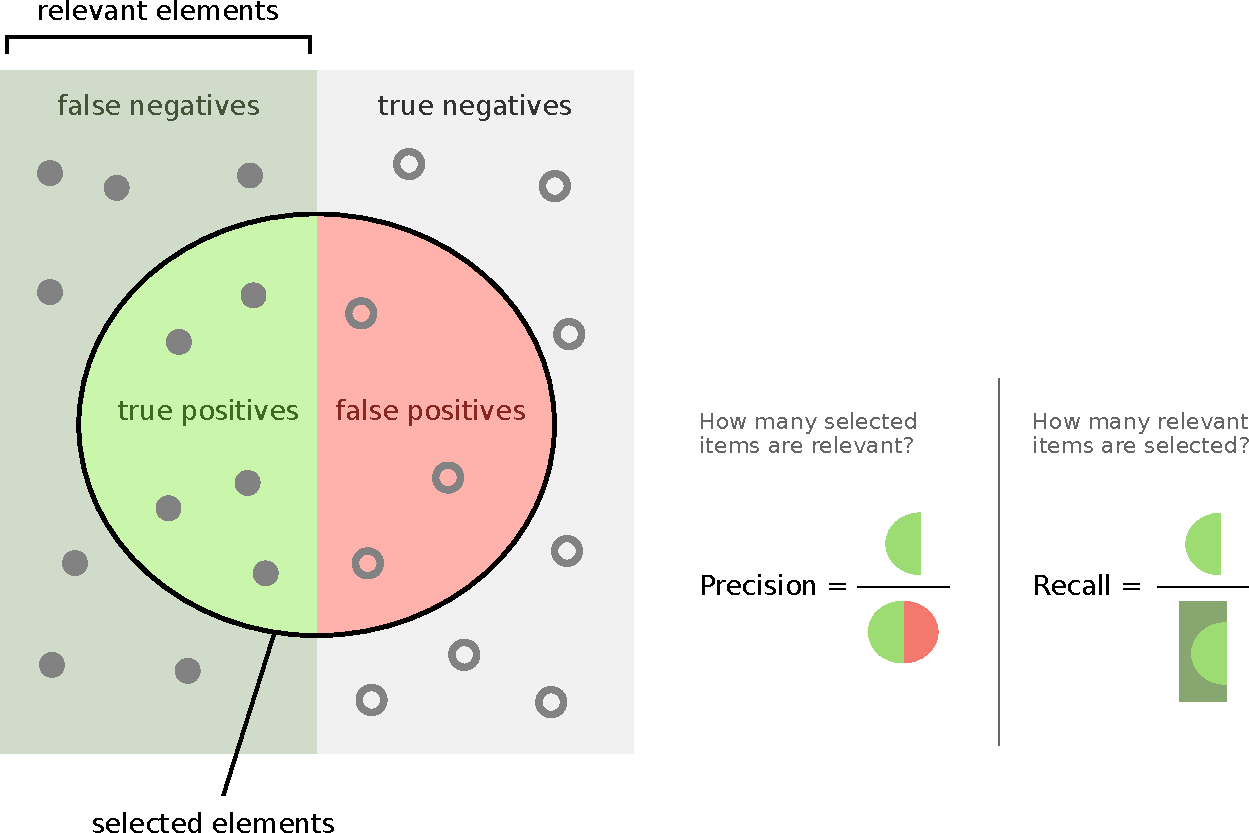
\includegraphics[width=0.7\textwidth]{./Bilder/Precisionrecall.pdf}
\caption[Precision and Recall]{Precision and Recall}
\label{fig:Pipeline}
\end{figure} 


%Quelle für recallprecisionBild: By Walber - Own work, CC BY-SA 4.0, https://commons.wikimedia.org/w/index.php?curid=36926283

%For determining the Receiver-Operating-Characteristic-Curve a True-Positive-Rate (TPR) and a False-Positive-Rate (FPR) is calculated.\\
%\begin{defn}\textbf{True-Positive-Rate (TPR).}The TPR values are for the y-axis of the ROC.
%\begin{equation}
%TPR=\frac{TP}{TP+FN}
%\end{equation}
%\end{defn}
%\begin{defn}
%\textbf{False-Positive-Rate (FPR).}The FPR values are for the x-axis of the ROC.
%\begin{equation}
%FPR=\frac{FP}{FP+TN}
%\end{equation}
%\end{defn}



\begin{defn}\textbf{Accuracy\\}
Accuracy is the percentage of correct predictions.
\begin{equation}
Accurancy=\frac{\text{Number of correct predictions}}{\text{Total number of predictions}}= \frac{TP+TN}{TP+TN+FP+FN}
\end{equation}
\end{defn}

Accuracy is not always an appropriate scoring method, because, assigning every object to a larger set achieves a high proportion of correct predictions, but is not generally a useful classification. For this reason Blanced Accuracy and the Mathew Correlation Coefficient are introduced.

\begin{defn}\textbf{Balanced Accurancy (BACC)}\\
Balanced Accuracy (BACC) is the Fraction of predictions our model got right divided by $2$.
\begin{equation}
BACC=\frac{\frac{\text{Number of correct predictions}}{\text{Total number of predictions}}}{2}= \frac{\frac{TP+TN}{TP+TN+FP+FN}}{2}
\end{equation}
\end{defn}

\begin{defn}\textbf{Matthew Correlation Coefficient (MCC)} \\
The MCC measures the quality of binary classifications and is a correlation coefficient between observed and predicted binary classifications which returns a value between $-1$ an $1$; $\text{MCC}\in [-1,1]$. Where a value close to $1$ denote a perfect prediction, a value close to $0$ means that the prediction is not better than a random one and a value close to $-1$ describes a total disagreement between prediction and observation.
\begin{equation}
\text{MCC= }\frac{TP*TN-FP*FN}{\sqrt{(TP+FP)(TP+FN)(TN+FP)(TN+FN)}}
\end{equation}
\end{defn}
%Quelle noch hinzufügen


\begin{exmp}
%https://developers.google.com/machine-learning/crash-course/classification/accuracy
Given is a model that classified 100 tumors as malignant (the positive calss) or benign (the negative class):
\begin{table}[!h]
\begin{center}
\begin{tabular}{ll}
\cellcolor{green!20}\begin{tabular}[c]{@{}l@{}}\textbf{True Positive (TP):}\\\begin{tabular}{@{\labelitemi\hspace{\dimexpr\labelsep+0.5\tabcolsep}}l}Reality Malignant\\Prediction: Malignant\\\textbf{Number of TP: 1}\end{tabular}\end{tabular} & \cellcolor{red!20}\begin{tabular}[c]{@{}l@{}}\textbf{False Posotive (FP):}\\\begin{tabular}{@{\labelitemi\hspace{\dimexpr\labelsep+0.5\tabcolsep}}l}Reality: Benign\\Prediction: Malignant\\\textbf{Number of FP: 1}\end{tabular}\end{tabular}  \\
\cellcolor{red!20}\begin{tabular}[c]{@{}l@{}}\textbf{False Negative (FN):}\\\begin{tabular}{@{\labelitemi\hspace{\dimexpr\labelsep+0.5\tabcolsep}}l}Reality: Malignant\\Prediction: Benign\\\textbf{Number of FN: 8}\end{tabular}\end{tabular}  & \cellcolor{green!20}\begin{tabular}[c]{@{}l@{}}\textbf{True Negative (TN):}\\\begin{tabular}{@{\labelitemi\hspace{\dimexpr\labelsep+0.5\tabcolsep}}l}Reality: Benign\\Prediction: Benign\\\textbf{Number of TN: 90}\end{tabular}\end{tabular}    
%\caption{Confusion matrix displaying all four possible outcomes.}
\end{tabular}
\caption{Confusion matrix displaying all four possible outcomes.}\end{center}
\end{table}

The confusion matrix in Table 2.3 shows that only one malignant tumor and $90$ not malignant tumors were predicted right by the model and $8$ tumors were predicted wrongly being benign and one being wrongly malignant. Now the performance of the model is calculated:

\begin{align}
Accuracy   = & \frac{1+90}{1+90+1+8}  = 0.91\\
Precision  = & \frac{1}{1+1}  = 0.5\\
Recall     = & \frac{1}{1+8}  = 0.11\\
TPR        = & \frac{1}{1+8} = 0.11 \\
FPR        = &  \frac{1}{1+90}  = 0.01  \\
BACC       = & \frac{\frac{1+90}{1+90+1+8}}{2} = 0.46  \\
MCC        = & \frac{1*90-1*8}{\sqrt{(1+1)(1+8)(90+1)(90+8)}}  = 0.21
\end{align}


The $Accurary$ (2.16) has a value of $0.91$ which means 91\% of the 100 total examples are predicted correctly. This result may look good at first sight, but this dataset is class-imbalanced. In a class-imbalanced data set the labels of a binary classification problem have significantly different frequencies. For example, a disease data set in which $0.0001$ of the examples have positve labels and $0.9999$ have negative labels is a class-imbalanced problem. But a football game predictor in which $0.51$ of example label one team winning and $0.49$ label the other team winning is not a class-imbalanced problem.\\
Thus the significant disparity between the number of positive (here: $TP+TN=91$) and negative labels (here: $FP+FN=9$) falsifies the result. This observation is supported by the values of the $BACC$ and the $MCC$. The $BACC$ (2.21) has a value of $0.46$, telling us that the prediction of the model is not that good as the $Accurary$ shows and the $MCC$ (2.22) has a value of $0.21$ which is quite close to a value of $0$. Thus the model predicted rather randomly than significantly. Furthermore the model has a $Precision$ of $0.5$, meaning when it predicts a tumor is malignant, it is correct $50\% $ of the time. The $Recall$ results in a value of $0.11$, meaning the model correctly identifies $11\%$ of all malignant tumors. In relation to this example it is worthwhile to identify most of the malignant tumors (high $TP$ value) and get a low number of unidentified malignant tumors (low $FN$ value). 
\end{exmp}
%Vielleicht hier besser ein Imbalance Beispiel für ein kleines Netzwerk zeigen.!!!!!
%Vielleicht noch eine metrik für dynamical accuracy hinzufügen (siehe: A mutual information-based Boolean network inference method)


\newpage
\section{Data collection: \textit{In silico} data set}
%Bild von der Pipeline


Before an inference algorithm and discretization method is applied to a real-life data set it is necessary to assess the performance.  Several methods are known to generate an \textit{in silico} data set, such that it was first tried to generate the \textit{in silico} data set independant on a real life organism, by applying the Barabasi-Albert (BA) model [Quelle[22]] or generate multiple sets from one exmaple network.\\
%Vllt. verweis zm git
The more sufficient method turned out to be creating an \textit{in silico} data set by extracting subnetworks from the E.Coli network. E.Coli (Escherichia coli) is a well studied bacterium consisting of 1565 genes (resp. nodes) with 3758 interaction (resp. edges). The subnetworks extracted from E.Coli are generated by a tool, called GeneNetWeaver 
%\cite{Gdoi:10.1093/bioinformatics/btr373}
. A set of four networks with 10 to 14 nodes, each extended to 9 subnetworks, such that 45 networks are yielded. For example a subnetwork of E.Coli can have a set of 10 nodes with a maximal in-degree of $indegree\in\{1,...,9\}$. The range of 10 to 14 is selected due to the fact, that REVEAL is not performing by a system of 15 nodes and starting by 10 is for better comparison of the perfomance measurement to literature [PaperQuelle].

\begin{figure}[H]
\captionsetup{width=0.8\linewidth}
\centering
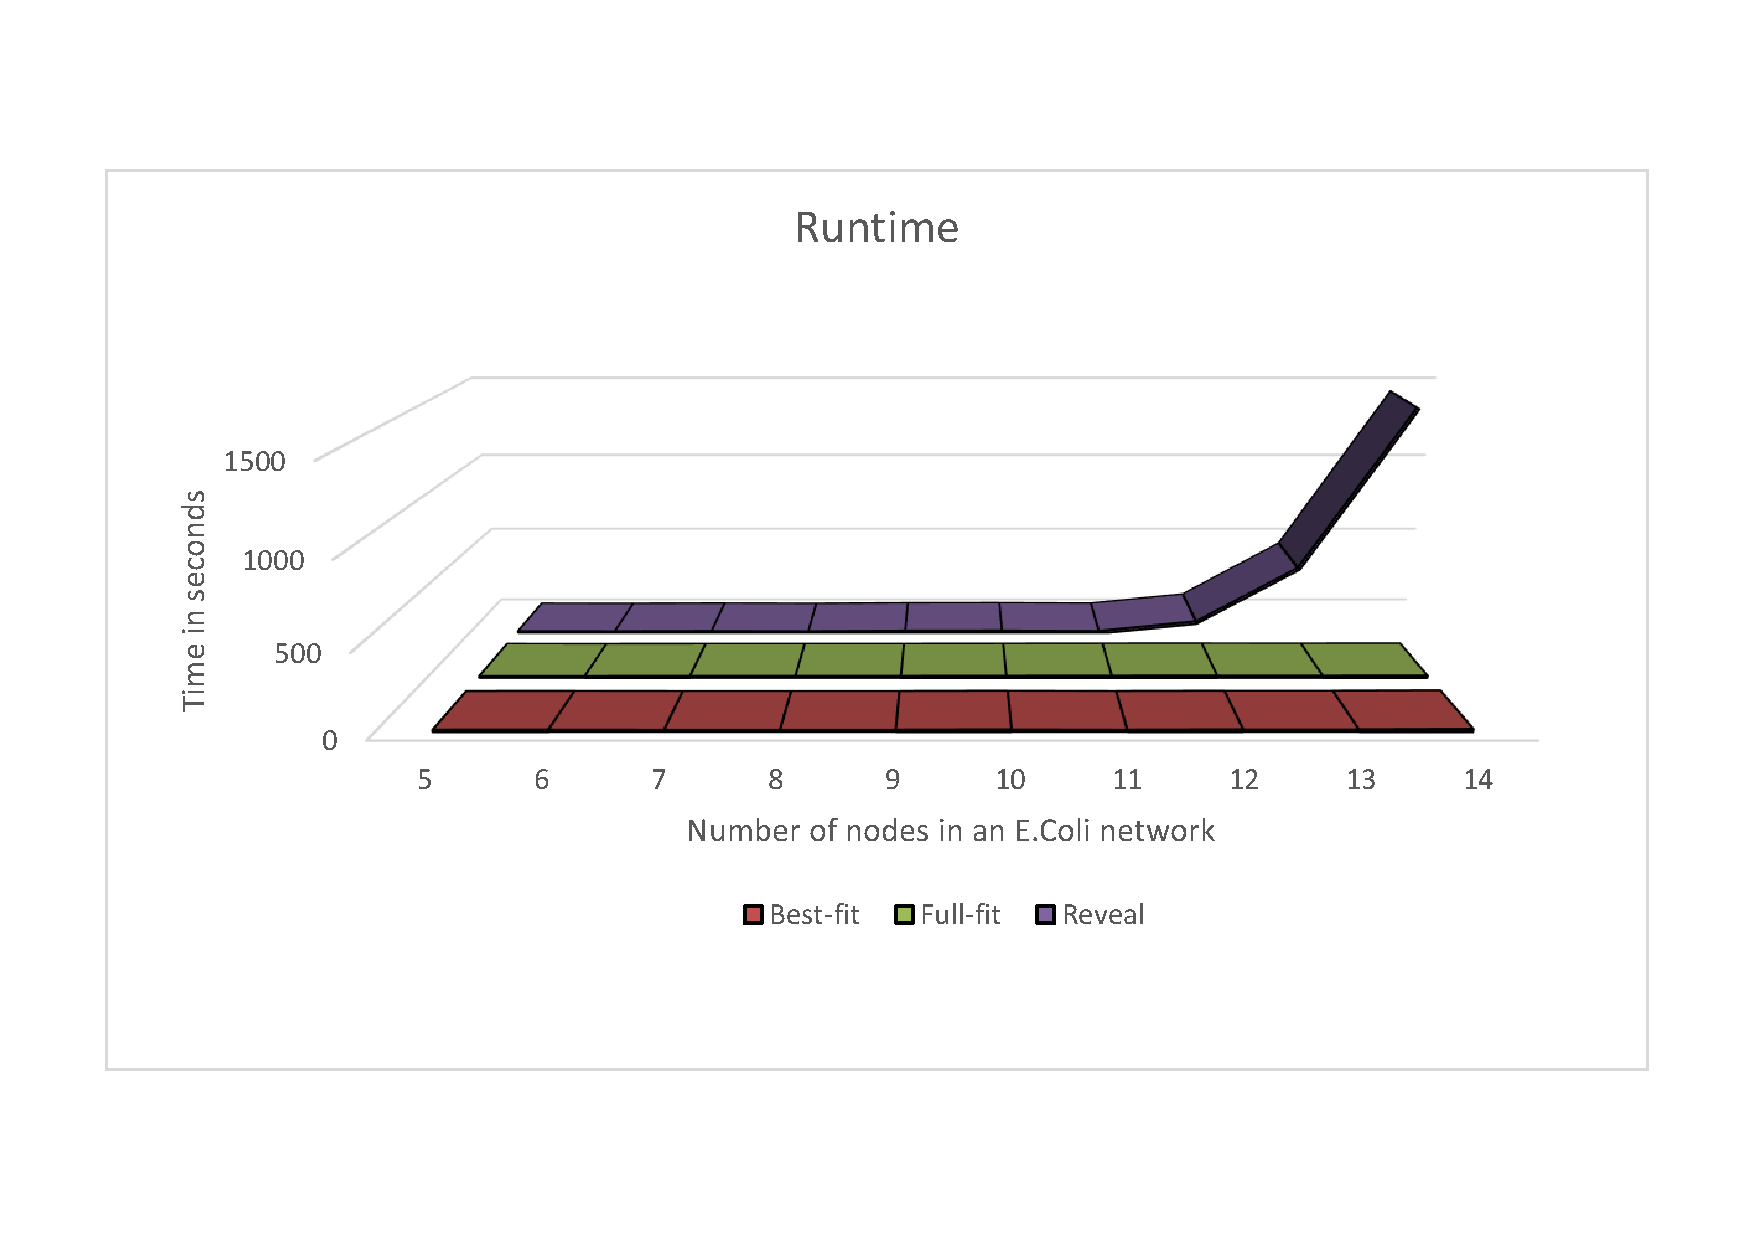
\includegraphics[width=0.9\textwidth]{./Bilder/Scoring/insilico/1_Indegree_Runtime/Runtime_nodes.pdf}
\caption[Runtime of Boolean Network Inference algorithms]{Starting by subnetworks of E.Coli of 5 nodes to a network of 14 nodes REVEAL is running out of time.}
\label{fig:}
\end{figure}

These networks help to figure out which algorithms performs the best by increasing the number of incoming links of a node. The number of incoming links represent the degree of complexity of the inference problem.\\
%\citep{doi:10.1093/bioinformatics/btw682}.
%\cite{doi:10.1093/bioinformatics/btl210}.
In addition a small real-life network of the mammalian cell cycle is used to asses the performance of the algorithms regarding the number of measurements and the clustering depth in the discretization step (Figure 2.4). The cell cycle network is taken from the repository of PyBoolNet. PyBoolNet is a python package for the generation, analysis and visualization of Boolean networks.\\
%Quelle: hannes Klarner Paper zu PyBoolNet
The cell cycle is a process of signal transduction leading to the reproduction of the genome of a cell (Synthesis or s phase ) and its division into daughter cells (Mitosis, or M phase). Positive signals or growth factors cause the activation of Cyclin D (CycD) in the cell, which inhibits the retinoblastoma protein Rb. Rb is a key tumor suppressor, which is mutated in large variety of cancer cells.
%Quelle: https://watermark.silverchair.com/btl210.pdf?token=AQECAHi208BE49Ooan9kkhW_Ercy7Dm3ZL_9Cf3qfKAc485ysgAAAkgwggJEBgkqhkiG9w0BBwagggI1MIICMQIBADCCAioGCSqGSIb3DQEHATAeBglghkgBZQMEAS4wEQQMkpP0kuTMdR7SdnuBAgEQgIIB-9YNfvnwOozBQbTwdM-qDZNJbor1i-sTBhi9eBu_buCn-a3LXScoKSPIJnVq6X5fbRPX1x6TO50sSRP65ov5XPCx3ZxUsCf5z1RWsvIxLXezJotwo40A9xBDfri6fRBVlCpS14gCumiBbUHnWFXmIiOSHUvnGhU7nvSMtXaCRYdUc6qtlkBoWoxfRIIjTlLp79OF3LSspQ7LDYqvtbiQRKEqdkHBabr1W2QaHG0GQ4Kk3hdX36yO5ZSGbJSNtd-SJsBpjfZ5niERUpLUDaUlv0MHzl1r7nVjn_O17-YWdqiVbyPaWdL0VFHcemLzYfFdx7Y4ao-kY81QA66CL8xFKqG1_j39ywpm3CzdPF0Uj0yT8OrZGdLkDcdnncY_Z8U8Xh_ZJ6zP_iI6pa74MBqH87pKcALmkz5WrPy4oLBW9bUl4yRyZ3YzEBnxLKt_ypqOzwyCAX5le0Q0mZ5-4hN8IJKGnohlb4hd2alda18evVDHGYfjU8g_FEVFAFQo227W4jV6QSeghgxW22uRrT6xNqagGqyx0kPrGidfvaON7E2a571yU8wE3JD__xmUE9An1YmxtHiGACmIsxEr2vFqJg_oJIzpnNsJdLshDXHq-P-45iWG-Gf-zW9PRS4qGaf4BhzAQfxUR7AevmWGPPt4DM6Iahkb4BCvJmlZJg
This cell cycle network consist of 10 interacting transcriptional counterparts of genes with 35 edges and has a maximal in-degree of 5. Therefore this network is an appropriate network to test the algorithms with.
%Bild von dem Interactiongraph von CellCycle
\captionsetup{width=0.8\linewidth}
\begin{figure}[H]
\centering
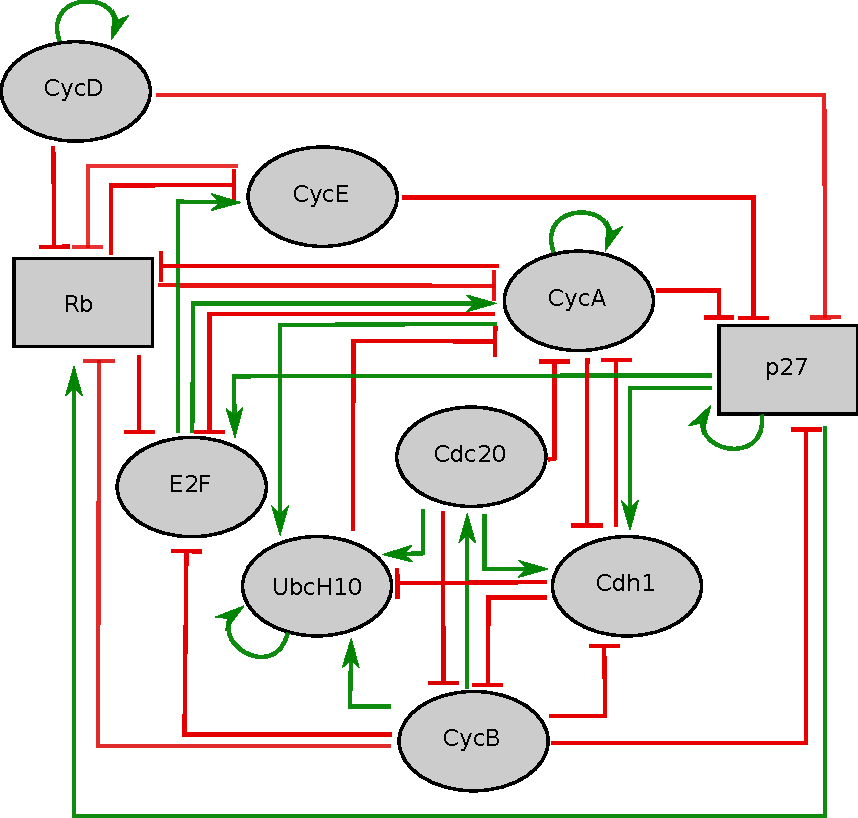
\includegraphics[width=0.6\textwidth]{./Bilder/cellcycle.pdf}
\caption[Cell cycle]{\textbf{Cell Cycle.} Logical regulatory directed graph for the mammalian cell cycle network. Each node represents a key regulatory element and each edge the interaction between them. Arrows describe activating activity (green) while blunt arrows describe inhibitory activity (red).}
\label{fig:9}
\end{figure}
%kurz cellcycle in biologischer funktion erklären
%Tabelle der funktionen der einzelnen Komponenten im Supplementary?
\newpage
\section{Data collection: Real-life course time data set }
%What is the Dream Challenge about? Which Dream Challenge to shoose?

For a Boolean network inference of real-life time-course data, the data of a platform so-called Dialogue on Reverse Engineering Assessment and Methods (\gls{DREAM}) - Challenge is used. The DREAM-Challenge is a non-profit, collaborative community effort consisting of contributors from across the research spectrum of questions in biology and medicine. This organization was built in 2006 and publishes crowdsourcing challenges with transparent sharing of data, thus everyone can participate the challenge. The DREAM-Challenge has partnered with Sage Bionetworks, which provide the infrastructure by Sage Bionetworks Synapse platform to get access to the open collaborative data analysis. Overall the DREAM-Challenge is a helpful instrument to get real-life data, comparing results  and interact with other researchers all over the world, while contribute solutions to biological and medical questions.
%\citep{DreamChalleneg Homepage}.
%Kürzer,vllt. besser in die Introduction?

%Which challenge to choose?
The challenging question is to decide which Dream Challenge data set could be useful for inferring Boolean networks with the introduced algorithms. For inferring a Boolean network the desired data set should contain measurements of experiments with less pertubational information in a time-course context with at least 50 sample points, such that all of the three algorithms are applicable. 
The Dream5- Network Infernece Challenge is dealing with gene-gene interaction, providing test, training data sets and a gold standard of gene expressions seemed to be an appropriate candidate. But there is less time-course information and a high abundance of pertubation (\gls{e.g.}. knockout experiments, gene deletion experiments, applied drugs and enviromental pertubations and dosages of the dugs), such that inferring a network by considering these additional information is quite challenging. In contrast to the Dream5 Challenge the Dream8 Challenge provides microarray data with less pertubation information, here the application of eight stimuli, but enough sample points  by about $\sim $85 for in each data set. Therefore this Dream Challenge is selected.

\subsection{DREAM8 Challenge}
%Short sentence about the DREAM8 Challenge: What is the goal(medically and mathematically)?What sub challenge do I do?
The "DREAM 8 - HPN-DREAM Breast Cancer Network Inference Challenge" took place in 2016 and was running for 3 month. The challenge focuses on inferring causal signaling networks by detecting phosphoproteins on signalling downstream of receptor tyrosine kinase (RTK) in human cancer cell lines.
%Causal networks
Causal signaling networks contain causal edges which may represent direct effects or indirect effects that occur via unmeasured intermediate nodes. For example in Figure 3.3 the inhibition of a parent node A can change the abundance of the child node B described by a directed edge. If node A causally influences node B via measured node C, the causal network should contain edges from A to C and from C to B,but not from A to B (top). However, if node C is not measured (and is not part of the network), the causal network should contain edges from A to B (bottom). In both cases the inhibition of A will lead to a change in node B.
%\citep{Inferring causal molecular networks-empirical assessment through a community-based effort}

\begin{SCfigure}[][!h]
\begin{minipage}{0.4\linewidth}
%\vspace{-\baselineskip}
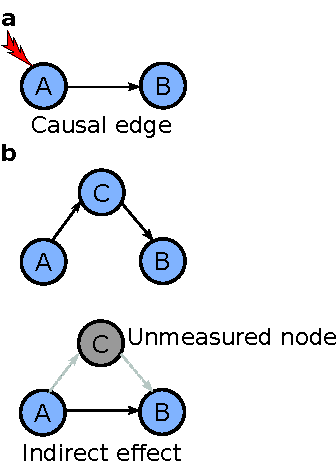
\includegraphics{./Bilder/causaledges.pdf}
\end{minipage}
\caption[Causal edges]{\textbf{Causal edges.} (a) Inhibition of a parent node A (red arrow) can change the abundance of child node B. (b) If node A influences B causually by measuring node C, then the causal network should contain edges from A to C and from C to B, but not from A to B. }
\label{fig:7}
\end{SCfigure}
%\citep{Pipeline}
%Graphik und caption an die Breite der seite anpassen
%Caption text soll unter der Figure-Bezeichnung stehen.




The real-life time-course data is provided by the Heritage Provider Network (HPN). More than 2000 networks were submitted by challenge participants. The networks spanned 32 contexts and were scored in terms of their structure and dynamics. 
The challenge shows that a significant network can be obtained by merging certain submitted network (submissions with high performance) to an aggregated network such that the community based approach proves that an aggregated network yields a higher performance in contrast to a single submission.
%Subchallenge description
The challenge comprised three sub-challenges: Causal network inference (SC1), time-course prediction(SC2) and visualization (SC3).
The sub-challenge SC1 is divided up into two parts A and B. In A the interaction graph with information about edge occurence is inferred and confidence score (resp. edge weights) indicating the strength of evidence in favour of each possible edge is calculated. Knowledge about the \textit{Sign} of an edge (i.e., wether activating or inhibitory) is neglected. In B the causal network is created and in the other two sub challenges the phosphoprotein time-course data is predicted under further pertubations and in the last challenge methods are developed to visualize these complex, multidimensional data sets. This work focuses on subchallenge SC1-A considering the inference of the interaction graph without taking the edge weight or \textit{Sign} into account. Thus the scability of the three inference algorithms from a small network to a big one can be assessed.

\subsection{Data structure}

%Biologicalinput data description
The challenge spanned 32 different contexts, each definded by a combination of 4 cell lines (BT20, UACC812, BT549, MCF7) and 8 stimuli (Insulin, Serum, HGF, NRG1,EGF, FGF1,GF1,IGF1)(Table 1.1) and three kinase inhibitors and a control DMSO (Dimethyl sulfoxide). The inhibitors inhibit the kinase activity of their target, which means they inhbit the ability of the target to catalyse phosphorylation of its substrates but not necessarily inhibit the phophorylation of the target itself.
%Quelle: https://www.synapse.org/#!Synapse:syn1720047/wiki/56061
All cell lines are provided by the American Type Culture Collection (ATCC) and where chosen because they represent the major subtypes of breat cancer (basal, luminal, laudin-low and HER2-amplified) and known to have different genomic abberations. 

%\citep{Neve, R. M., Chin, K., Fridlyand, J., Yeh, J., Baehner, F. L., Fevr, T., … Gray, J. W. (2006). A collection of breast cancer cell lines for the study of functionally distinct cancer subtypes. Cancer Cell, 10(6), 515–527. http://doi.org/10.1016/j.ccr.2006.10.008}
%\citep{https://www.nature.com/articles/nature11005}
%\citep{Barretina, J., Caponigro, G., Stransky, N., Venkatesan, K., Margolin, A. A., Kim, S., … Garraway, L. A. (2012). The Cancer Cell Line Encyclopedia enables predictive modeling of anticancer drug sensitivity. Nature, 483(7391), 603–607. http://doi.org/10.1038/nature11003}
%\citep{https://clinicalproteomicsjournal.biomedcentral.com/articles/10.1007/s12014-010-9055-y}
\subsection*{Experimental setting}
Protein arrays were carried out using RPMA, an antibody detection method described in the biological background in chapter 1. Each cell line was serum-starved for 24hours and then treated for 2 hours with an inhibitor (or combination of them). Cells were then either harvested (0 time point) or stimulated by one of the eight stimuli for 5, 15, 30 or 60 minutes or for 2 or 4 hours (Figure 2.6).
%picture of the treatment: https://www.synapse.org/#!Synapse:syn1720047/wiki/56061
\begin{SCfigure}[][!h]
\begin{minipage}{0.5\linewidth}
%\vspace{-\baselineskip}
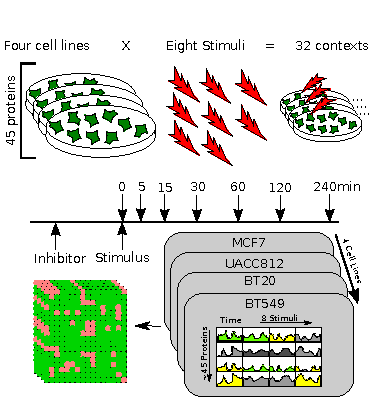
\includegraphics{./Bilder/datacollectiondream8.pdf}
\end{minipage}
\caption[Data Collection of the Dream8 Challenge data set]{\textbf{Data collection.} Four cell lines (MCF7, UACC812, BT20, BT549) are treated with eight stimuli resulting in 32 contexts. Every experiment starts by adding an inhibitor followed by a stimlus. The concentration of 45phosphoprotein detecting antibodies is measured after 5,15,30,60,120 and 240 minutes. }
\label{fig:7}
\end{SCfigure}




%Data structure
In each of the 32 contexts time-course data for $\sim$ 45 phophoproteins measured up to four hours depicted as the 'main-data set'. The number of measured phophoproteins varies across the cell lines due to the antibodies, which evolve over time during the experiments. Participants who were interested in more phosphoproteins and more sample points were referred to a 'full-data set' with measurements up to 72 hours and an amount of up to 125 phophoproteins. %\citep{https://www.synapse.org/#!Synapse:syn1720047/wiki/56061}.
As in the challenge the inference is focused on the 'main data set', which is here the training data set. The provided data (for each of the 32 contexts) is contained in a Comma Seperated Values (\gls{CSV}) file format.
\subsection*{Normalization}
The data is normalized by converting raw data from $log_2$ values to linear values. For each antibody across the sample set the median is determined. The median value denote the middle position when all the observations are arraged in an ascending or descending order. It divides the frequency distribution exactly into two halves. Fifty percent of observations in a distribution have scores at or below the median. Hence median is the 50th percentile and also known as the 'positional average'.
%MedianQuelle: Measures of central tendency: Median and mode
Each raw linear value is divided by the median to get the median-centered ratio. Then the median of the median-centered ratio is calculated for each sample across the entire amount of antibodies. This median functions as a correction factor, thus each sample has its own correction factor. If the correction factor is above a value of 2.5 or below a value of 0.25 then the sample is considered as an outlier and extracted from the data set. Finally each median-centered ratio is divided by the correction factor resulting in normalized linear values.\\
%Quelle: https://www.synapse.org/#!Synapse:syn1720047/wiki/56061 
%Normalization: on linear scale: https://en.wikipedia.org/wiki/Feature_scaling 
%PaperQuelleNCBI: A Comprehensive Comparison of Normalization Methods for Loading Control and Variance Stabilization of Reverse-Phase Protein Array Data
\subsection*{Training data}
A \gls{CSV} file is structured by four headers starting with the 'Slide ID' containing information about the protein name, it's phospholylation site, antibody type, antibody validation status, and the antibody slide number (Table 2.8). The 'Antibody Name' describes the protein name, the phosphorylation site and antibody type (e.g.,Antibody name: '4EBP1$\_$ pT37$\_$pT46', where '4EBP1' depict the phophoprotein). The third header is a 'HUGO ID' an approved nomenclature of the proteins in combination with the the phosphorylation site. For the network inference the Anibody names are depicted as the node names in a network.
The last header shows the type of a cell line, the inhibitor, the stimulus, the timepoint of measurement followed by the concentration measured for each phosphoprotein detecting antibody.
%Show structure of Main CSV data\\
\begin{table}[!h]
%\resizebox{\textwidth}{!}{
{\tabcolsep=3pt%
\begin{center}
%\captionsetup{width=0.87\linewidth}
\scriptsize
\begin{tabular}{llllll}
\toprule 
 & & & \textbf{Slide ID} & 4E-BP1$\_$pT37$\_$T46-R-V$\_$GBL9026591 & ... \\
\toprule
 & & & \textbf{Antibody Name} & 4EBP1$\_$pT37$\_$pT46 & ... \\
\toprule
 & & & \textbf{HUGO ID} & EIF4EBP1$\_$pT37$\_$pT46 & ... \\
\toprule
 \textbf{Cell Line} & \textbf{Inhibitor} & \textbf{Stimulus} & \textbf{Timepoint} & & \\
\hline
\rowcolor{black!10} BT20 & Inhibitor &   & 0 & 3.0724988347 & ...\\
 					BT20 & Inhibitor	& 	& 0 & 3.168004721 & ...\\
\rowcolor{black!10} BT20 & Inhibitor	&	& 0	& 3.0629789682	& ...\\
 					BT20 & ...	&	& ... & ...	& ...\\
\rowcolor{black!10} BT20 &	& Insulin	& 5	& 3.3041031492	&...\\
 					BT20 & 	& FGF1 &	5 & 4.315396736	& ...\\
\rowcolor{black!10} ... &	...	& ... &	...	& ...	& ... \\
\bottomrule
\end{tabular}
\captionof{table}{Table of \gls{CSV} file}
\end{center}
}
\end{table}

%Problem: Tabl is out of range!!!






